%%%%%%%%%%%%%%%%%%%%%%%%%%%%%%%%%%%%%%%%%%%%%
\subsubsection{Open Heavy Flavor Dynamics}
	\label{Sec:OpenHF}
%%%%%%%%%%%%%%%%%%%%%%%%%%%%%%%%%%%%%%%%%%%%%

 The diffusion of a heavy particle through a heat bath of light particles can be 
 quantified by the spatial diffusion coefficient $D_s$. In 
 relativistic systems, such as the QGP, it is convenient to express this transport 
 coefficient in units of the thermal wavelength of the medium, $1/2\pi T$. This renders 
 $D_s(2\pi T)$ a dimensionless quantity which characterizes the (inverse) coupling 
 strength of the diffusing particle to the medium. As such, it is expected to be 
 proportional to the ratio of shear viscosity to entropy, $\eta/s$. For example, in 
 the strong coupling limit of conformal field theories, one has 
 $D_s(2\pi T) \simeq 1$~\cite{Herzog:2006gh,CasalderreySolana:2006rq} and 
 $\eta/s=1/4\pi$ (where small values for each of these quantities indicate strong coupling). 
 
In contrast to the result for strongly coupled theories, perturbative systems
generate much large values for the heavy quark diffusion coefficient. For example,
early calculations based on perturbative methods of the diffusion coefficient for charm and bottom quarks in 
 a QGP~\cite{Svetitsky:1987gq} produced values 
 of $D_s(2\pi T) \simeq 30 \sim {\cal O}(1/\alpha_s^2)$ for a strong coupling 
 constant of $\alpha_s\simeq$~0.3-0.4,  and with a value varying only weakly with temperature. 
 We now know from a 
 phenomenological point of view that these values for $D_s$ are too large to account for 
 the open heavy-flavor (HF) observables in heavy-ion collisions at RHIC and 
 the LHC~\cite{Rapp:2009my}. Later it was found that the formal convergence of the 
 perturbative series requires much smaller values for $\alpha_s$~\cite{CaronHuot:2008uh}. 
 This calls for nonperturbative methods to assess the heavy-flavor diffusion 
 coefficient in QCD matter.  
 
 \begin{figure}[tbh]
 \centerline{ 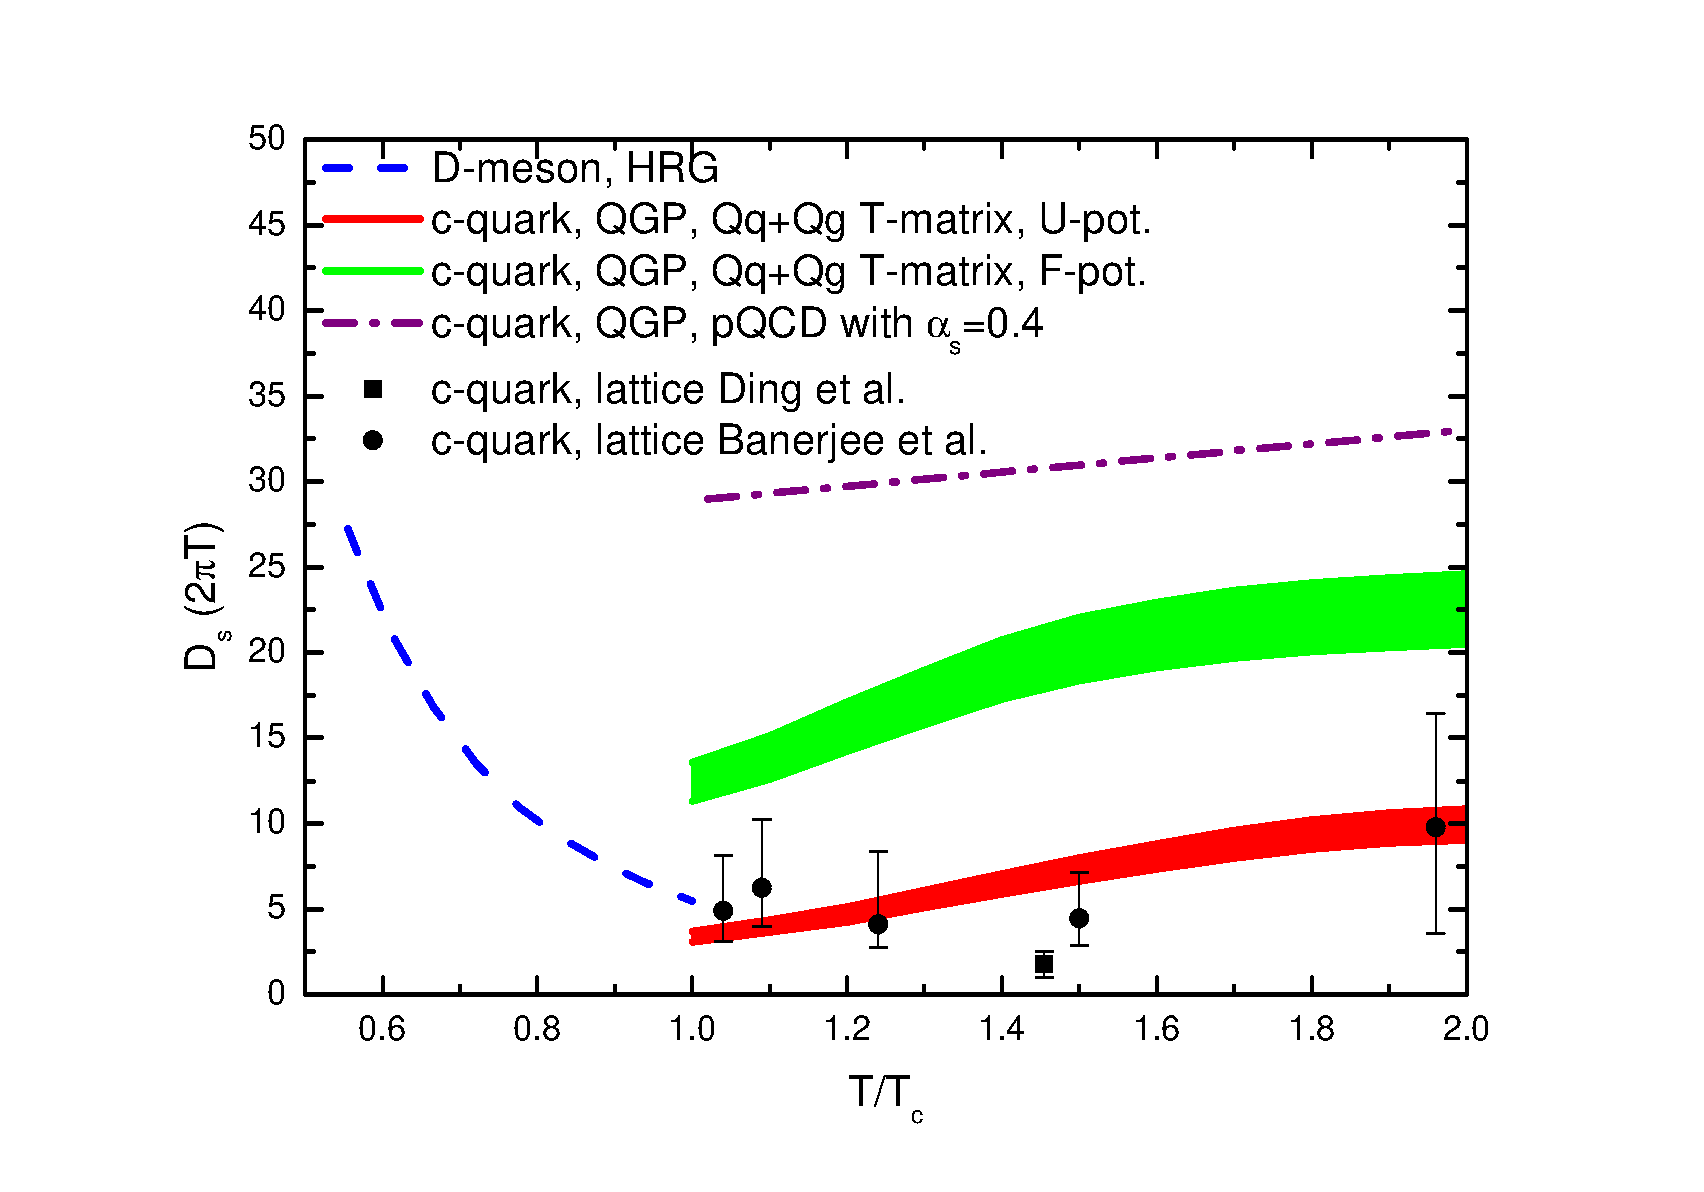
\includegraphics[width=1.00\textwidth]{fig/Ds-2piT} }
 \caption[Spatial diffusion coefficient for charm quarks and $D$-mesons]{Spatial diffusion coefficient for charm quarks in the QGP ($T>T_{\rm c}$)
 and $D$-mesons in hadronic matter ($T<T_{\rm c}$), in units of the thermal wavelength.
 The data points are extracted from quenched 
 lattice QCD~\cite{Banerjee:2011ra,Ding:2012sp,Kaczmarek:2014jga} while the bands are 
 obtained from potential-based $T$-matrix calculations~\cite{Riek:2010fk,Huggins:2012dj} 
 using either the free (green) or internal (red) energies from lattice QCD. The dash-dotted 
 line corresponds to leading order perturbation theory~\cite{Svetitsky:1987gq}.
 }
 \label{fig:Ds-2piT}
 \end{figure}
 Progress has been made to extract $D_s$ from first principles in thermal lattice QCD, 
 by computing euclidean heavy-quark (HQ) correlation functions and reconstructing the 
 low-energy limit of the pertinent spectral function (which defines the transport coefficient). 
 Thus far this has been done in quenched QCD (i.e., in a gluon plasma without dynamical 
 quarks)~\cite{Banerjee:2011ra,Ding:2012sp,Kaczmarek:2014jga}, resulting in a range of 
 values of $D_s(2\pi T) \simeq$~2-6 for temperatures between 1-2~$T_c$, as shown in 
 Figure~\ref{fig:Ds-2piT}. 
 To make closer contact to experiment, it will be necessary to extend these studies 
 to QCD with dynamical quarks, and to compute the 3-momentum dependence of the transport 
 coefficient. The latter can be alternatively expressed through the thermal relaxation 
 rate, $\gamma_Q=T/(m_Q D_s)$, where $m_Q$ is the HQ mass in the QGP, or heavy-meson mass 
 in hadronic matter. 
 
 Non-perturbative calculations of the HQ transport coefficients have also been carried out 
 in the thermodynamic $T$-matrix formalism~\cite{vanHees:2007me,Riek:2010fk,Huggins:2012dj}, 
 which is based on a potential approximation for HQ scattering off thermal partons. The 
 in-medium potential can, in principle, be extracted from thermal lattice QCD, see, e.g., 
 Ref.~\cite{Burnier:2014ssa}. Current uncertainties are usually bracketed by employing 
 either the HQ internal or free energies from the lattice. Using the internal energy one 
 finds values of $D_s(2\pi T)\simeq$\,3-5 at temperatures close to $T_{\rm c}$, increasing 
 to about 10 at 2\,$T_{\rm c}$, for both charm and bottom quarks, see Figure~\ref{fig:Ds-2piT}. 
 For the free energy, the $D_s$ values are about a factor of 2-4 larger. The relaxation 
 rates from the $T$-matrix formalism predict an appreciable 3-momentum dependence, decreasing 
 toward perturbative values at high momenta. Close to $T_{\rm c}$, resonant structures develop 
 in the heavy-light quark $T$-matrices, suggestive of the onset of hadronization. 
 
 Recent work has demonstrated the importance of also treating the  $D$ meson diffusion in the hadronic 
 phase. The pertinent transport coefficient has been estimated 
 in heavy-meson chiral perturbation theory~\cite{Laine:2011is} and in effective 
 hadronic theories including resonance 
 scattering~\cite{He:2011yi,Ghosh:2011bw,Abreu:2011ic,Tolos:2013kva}. The $D$-meson 
 diffusion coefficient significantly decreases as $T_{\rm c}$ is approached from below. 
 There is increasing consensus that its hadronic values~\cite{He:2011yi,Tolos:2013kva} 
 come close to the nonperturbative approaches on the QGP side. This suggests that the 
 heavy-flavor diffusion coefficient develops a minimum across the phase transition 
 region, with a near-continuous temperature dependence when passing from hadronic 
 to partonic degrees of freedom, as one would expect in a cross-over 
 transition~\cite{He:2011yi,He:2012df,Tolos:2013kva}. 
 
 \begin{figure}[tbh] 
 \centerline{ 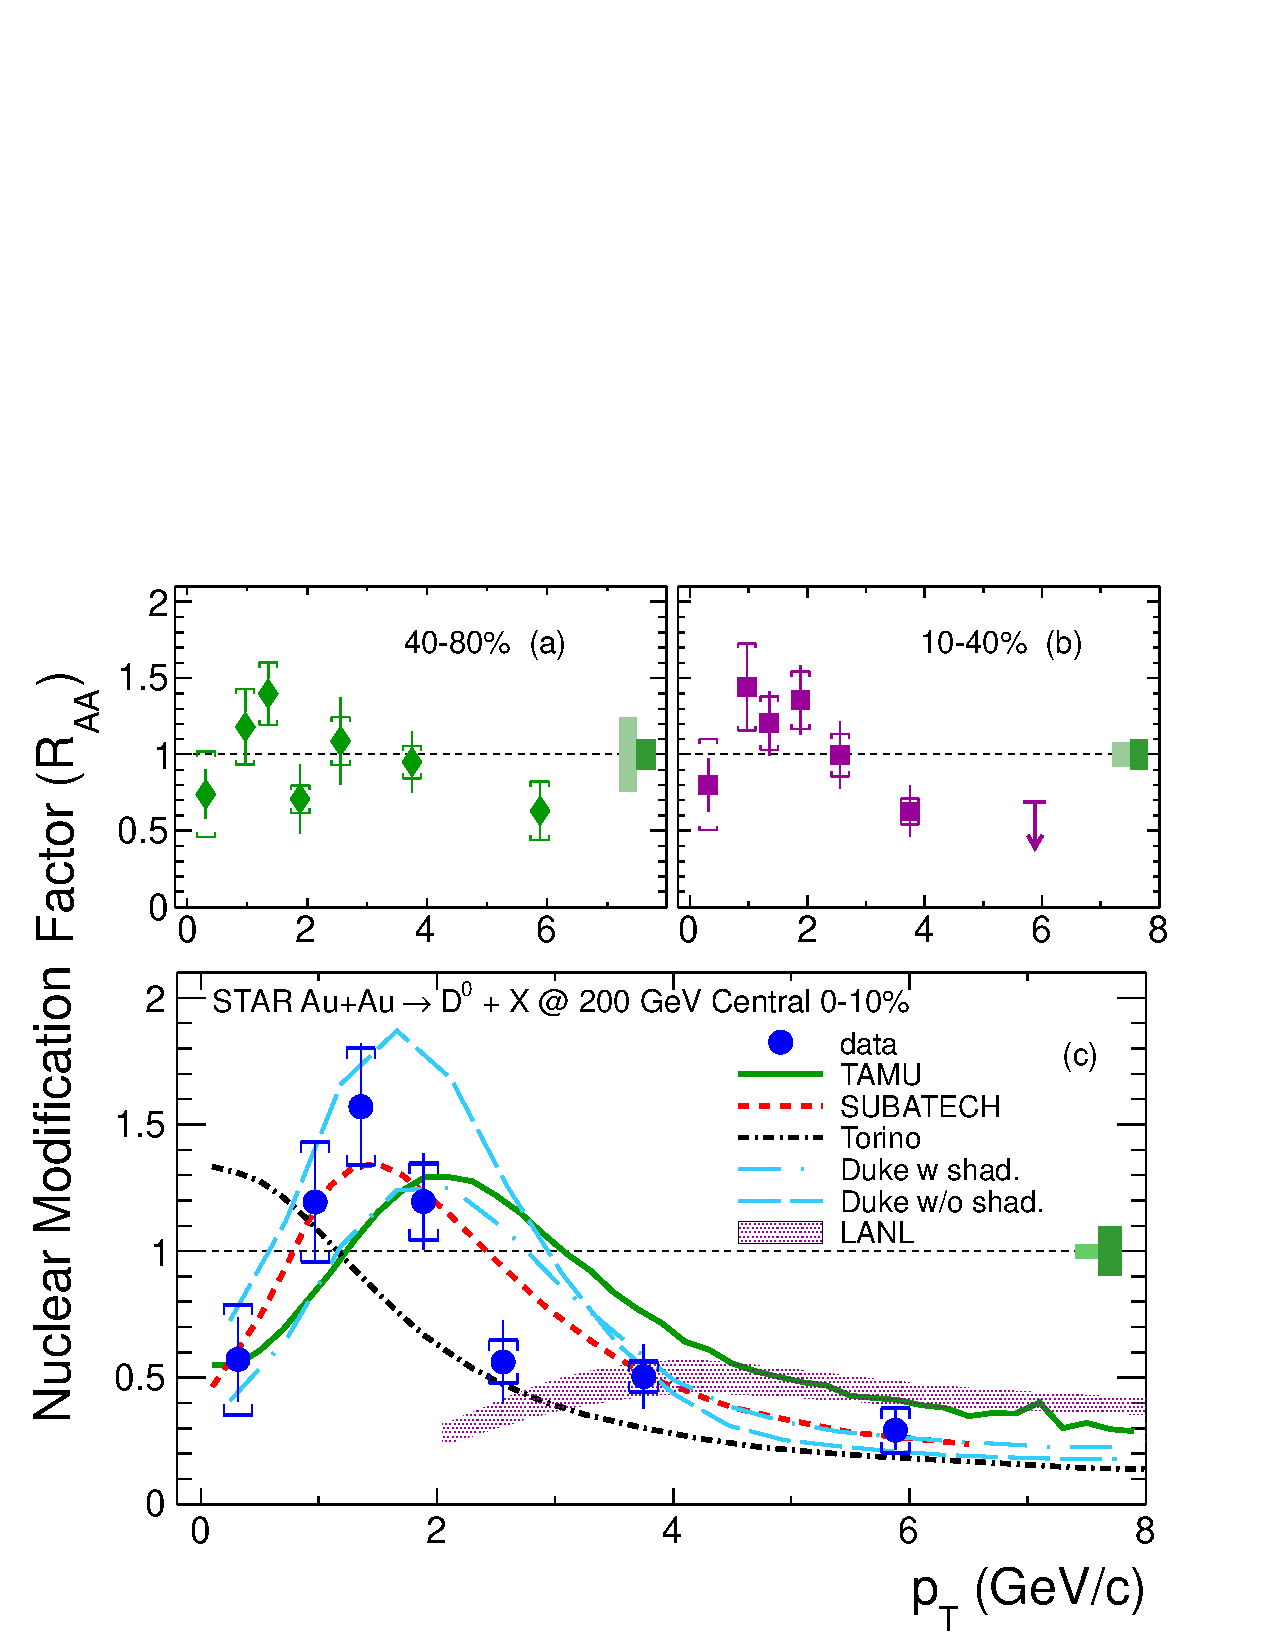
\includegraphics[width=0.90\textwidth]{fig/D-RAA-star} } 
 \caption[STAR measurements of $D$-meson production compared to theory]{Nuclear modification factor of $D$-mesons in 200 GeV \AuAu\ collisions 
 at various centralities as measured by STAR~\cite{Adamczyk:2014uip}, compared to 
 theoretical 
 calculations~\cite{Adil:2006ra,Gossiaux:2008jv,He:2011qa,Alberico:2013bza,Cao:2013ita} 
 } 
 \label{fig:D-RAA-star} 
 \end{figure} 
 Remarkable results for open heavy-flavor observables have recently been obtained at 
 both RHIC and the LHC. The STAR~\cite{Adamczyk:2014uip} and 
 ALICE~\cite{Alice:2012ab,Abelev:2013lca,Abelev:2014ipa} collaborations have, for the 
 first time, been able to extract the nuclear modification factor ($R_{AA}$) and 
 elliptic flow ($v_2$) of $D$ mesons. The STAR measurement of $D$ mesons in 200 GeV 
 Au-Au reaches down to rather low transverse momenta ($p_T$)~\cite{Adamczyk:2014uip}, 
 showing intriguing evidence for a maximum in the $R_{AA}(p_T)$ as seen in 
 Figure~\ref{fig:D-RAA-star}. Such a structure is a tell-tale signature for collective 
 behavior of $D$ mesons, which in turn requires a strong coupling of $c$ quarks and $D$ mesons 
 to the expanding medium. As part of the thermalization process, the heavy-flavor
 particles are dragged along in the fireball expansion and accumulate in a momentum range
 characteristic of the medium's collective flow velocity, while low- and high-momentum states are 
 depleted. This feature can be described by theoretical calculations which implement 
 (a) a sufficiently small diffusion coefficient of $ D_s (2\pi T) \leq5$ into dynamical 
 evolution models~\cite{He:2011qa,Gossiaux:2008jv,Cao:2013ita}, and 
 (b) heavy-light 
 quark coalescence in the hadronization process. The precise location of the
 flow bump turns out to be rather sensitive to the underlying bulk evolution model. 
 Systematic comparisons of the different ingredients to the theoretical models and 
 improved precision in the data are required to disentangle the different effects and 
 arrive at quantitative results for the heavy-quark transport coefficient. 
 Additionally, measurements of the $R_{AA}$ of $D_s$ mesons (containing one charm and 
 one strange anti-/quark), would be very helpful as coalescence processes of $c$ quarks 
 with the enhanced strangeness content of the QGP significantly augment the flow 
 bump~\cite{He:2012df}.  

 A critical role in the determination of the transport coefficient is played by measurements of the elliptic flow parameter
 $v_2$ of the heavy-flavor particles. Electrons and muons from semileptonic decays 
 of $D$- and $B$-meson have been found to carry a rather large $v_2$ in heavy ion
 collisions at both RHIC~\cite{Adare:2006nq,Mustafa:2012jh} and the LHC~\cite{Sakai:2013ata}. 
 Important midterm goals at RHIC are to disentangle the $B$ and $D$ contributions to the semileptonic decays, and to 
 obtain an independent measurement of the $v_2$ of directly reconstructed $D$ mesons. 
 The former will be extracted from existing RHIC 2014 Au+Au displaced vertex 
 measurements by PHENIX (using the VTX and FVTX detectors)~\cite{Nouicer:2012pr}, and by 
 STAR (using the HFT detector)~\cite{Kapitan:2008kk,Qiu:2014dha}. The $v_2$ of directly reconstructed $D$ mesons 
 will be obtained from the same data set using the STAR HFT~\cite{Qiu:2014dha}. 
 At the LHC, ALICE has 
 conducted first measurements of the $D$-meson $v_2$ in 2.76\,TeV \PbPb\ 
 collisions~\cite{Abelev:2013lca}, and found large values; CMS has been able to extract 
 a $B$-meson $R_{AA}$ through their displaced-vertex decays into $J/\psi$'s (so-called 
 non-prompt $J/\psi$'s~\cite{Chatrchyan:2012np}, which is approximately unity for small  
 momenta and turns into a suppression leveling off at $\sim$0.5 at high momenta. As 
 in the $D$-meson sector, this is consistent with collective behavior and thus indicative 
 for a strong bottom coupling to the medium, providing further valuable model constraints.

 An outstanding  issue is the determination of the temperature dependence of the transport coefficient.  
 Experimentally, one lever arm is provided by the correlation between $v_2$ and the 
 $R_{AA}$. Since the bulk medium $v_2$ takes several fm/$c$ to build up, a large $v_2$ 
 of the HF particles is indicative for a strong coupling in the later QGP phases of the 
 fireball evolution, and through hadronization. 
 A suppression in the $R_{AA}$, on the other hand, begins immediately in the early 
 high-density phases, especially at high $p_T$. Model calculations to date
 cannot easily account for the large $D$-meson $v_2$ at LHC without overestimating 
 the suppression in the $R_{AA}$. This corroborates a strong coupling in the vicinity
 of $T_{\rm c}$. The second lever arm is provided by going to lower collision 
 energies where the system starts out at smaller QGP temperatures, closer to $T_{\rm c}$. 
 First data for the heavy-flavor electron $R_{AA}$ and $v_2$ have been extracted
 from a 62\,GeV run at RHIC~\cite{Adare:2014rly,Adamczyk:2014yew}, and show evidence 
 for a non-vanishing $v_2$ and marked modifications in the $R_{AA}$. They are not 
 imcompatible with model calculations that utilize a strong heavy-flavor coupling around 
 $T_c$~\cite{He:2014epa}, but the data precision does not yet suffice for clear conclusions. 
 While varying the collision energy is a valuable tool to explore the temperature 
 dependence of these phenomena, it is necessary to account for the 
 more pronounced role of the Cronin effect at these energies, i.e., 
 a modification of the heavy-flavor spectra through cold nuclear matter effects, before 
 the QGP forms. 
Here  \pA\ collisions will be important to quantify these effects in order to provide a realistic starting 
point for assessing the hot-medium effects. 
 
  

%\bibliographystyle{atlasnote}
%\bibliography{OpenHeavyFlavor}

%\end{document}

